\chapter{Gravitation}
\section{F and g}

\begin{definition}{Newton's Law of Universal Gravitation}{nlug}
	Every \it{point mass} attracts every other point mass with a force
	\begin{enumerate}
		\item directly proportional to the product of their masses
		\item inversely proportional to the square of the distance between them
	\end{enumerate}
	\[F = \f{GMm}{r^2} = -\odv{U}{r}\]
\end{definition}

\begin{definition}{Gravitational field strength}{grav-field}
	Gravitational force \it{per unit mass} acting on a small point mass
	placed at a point within a gravitational field
	\[g = \f{F}{m} = \f{G M}{r^2} = -\odv{\phi}{r}\]
\end{definition}

\bf{Gravitational field lines} are
\begin{itemize}
	\item \it{directed radially} towards a point mass
	\item \it{spreading out} at further distances from the point mass
\end{itemize}

\begin{example}{}{earth-g}
	The value of \(\va{g}\) varies at different points on Earth's surface, because
	\begin{itemize}
		\item the Earth is rotating
		\item the Earth is not a perfect sphere (bulges at the equator)
		\item the Earth's density is not uniform
	\end{itemize}
\end{example}

\begin{definition}{Weightlessness}{weightlessness}
	Sensation when \it{no physical contact force} acts on the body (e.g.~during free fall)
\end{definition}

\bf{Geostationary satellites} are those which
\begin{itemize}
	\item have a period of \qty{24}{\hour}
	\item have the same direction of rotation as the Earth (west to east)
	\item rotate in the plane containing the equator
\end{itemize}

\section{U and phi}
\begin{definition}{Gravitational potential energy}{gpe}
	Work done by an external force to bring a small test mass at infinity to
	a point within a gravitational field \it{with no change in k.e.}.
	\[U = -\f{GMm}{r} = \int^{r}_{\infty} \va{F} \odif{r}\]
\end{definition}

\begin{example}{}{negative-gpe}
	\it{Why is GPE negative?}
	\begin{itemize}
		\item \(\va{F}_g\) is attractive in nature
		\item To bring a mass from infinity to a point within a gravitational field, we must apply an external force \it{opposite} to \(\va{F}_g\)
		\item External force and mass's displacement are in \it{opposite directions} \(\implies\) the external force does \it{negative work}
	\end{itemize}
\end{example}

\begin{definition}{Gravitational potential}{grav-pot}
	Work done \it{per unit mass} by an external force to bring a small test mass
	from infinity to a point within a gravitational field, with \it{no change in k.e.}.
	\[\phi = \f{U}{m} = -\f{GM}{r} = \int^{r}_{\infty} \va{g} \odif{r}\]
\end{definition}
Moving a mass \(m\) from one point of potential \(\phi_i\) to another
point of potential \(\phi_f\) means that \(\Delta U = m\ab(\phi_f-\phi_i)\).
\term{The work done on the mass is \(W = -\Delta U\).}

\begin{marginfigure}
	\centering
	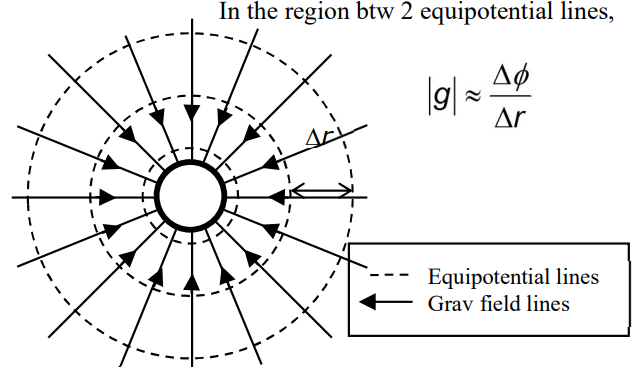
\includegraphics[width=\textwidth]{assets/g-phi.png}
	\label{fig:g-phi}
	\caption{\(g\) and equi-\(\phi\) lines}
\end{marginfigure}

\section{Other examples}
Let \(R \coloneq\) the radius of the Earth and \(M \coloneq\) its mass.
\begin{example}{Escape speed}{escape-speed}
	Projecting a mass \(m\) with an \bf{escape speed} \(v\) from the surface of the Earth
	will cause the mass to escape the Earth's \(g\)-field.
	For \(\min v\),
	\begin{align*}
		K_i + U_i                    & = K_f + U_f            \\
		\f{mv^2}{2}+\ab(-\f{GMm}{R}) & = 0                    \\
		\implies v                   & = \sqrt{\frac{2GM}{R}}
	\end{align*}
\end{example}

\begin{example}{Orbiting satellite}{orbiting-satellite}
	A satellite of mass \(m\) orbiting the Earth at a distance \(r\) from its centre
	with speed \(v\) will need gravitational force to provide its centripetal
	acceleration (\(F_g\) provides \(F_c\)).
	\begin{align*}
		\f{mv^2}{r}              & = \f{GMm}{r^2}     \\
		v                        & = \sqrt{\f{GM}{r}} \\
		\implies K = \f{mv^2}{2} & = \f{GMm}{2r}
	\end{align*}

	Total energy isn't conserved when the satellite moves from
	an orbit radius \(r_i\) to a new orbit radius \(r_f\).
	\begin{align*}
		K_i + U_i + W_{\text{ext}}                          & = K_f + U_f                              \\
		\f{GMm}{2r_i} + \ab(-\f{GMm}{r_i}) + W_{\text{ext}} & = \f{GMm}{2r_f} + \ab(-\f{GMm}{r_f})     \\
		-\f{GMm}{2r_i} + W_{\text{ext}}                     & = -\f{GMm}{2r_f}                         \\
		W_{\text{ext}}                                      & = \f{GMm}{2}\ab(\f{1}{r_i} - \f{1}{r_f})
	\end{align*}
\end{example}

\begin{example}{Binary star}{binary-star}
	For two stars \(m_1\) and \(m_2\) orbiting at radii \(r_1\) and \(r_2\) about a common centre,
	\(F_g\) provides \(F_c\) of either star.
	\begin{align*}
		\f{Gm_1m_2}{\ab(r_1+r_2)^2} & = m_1r_1\omega^2 = m_2r_2\omega^2 \\
		\implies \lf{m_1}{m_2}      & = \lf{r_2}{r_1}
	\end{align*}
\end{example}

\begin{figure}[htpb]
	\centering
	\input{assets/g-summary.tikz}
	\caption{Formulae}
	\label{fig:g-summary}
\end{figure}
